\section{Технический проект}
\subsection{Общая характеристика организации решения задачи}

Необходимо спроектировать и разработать систему тестирования, которая должна измерять качества и свойства личности.

Система тестирования представляет собой набор взаимосвязанных окон, которые сгруппированы по разделам, содержащие текстовую и графическую информацию. 

\subsection{Обоснование выбора технологии проектирования}

На сегодняшний день информационный рынок, поставляющий программные решения в выбранной сфере, предлагает множество продуктов, позволяющих достигнуть поставленной цели – разработки системы тестирования.

\subsubsection{Описание используемых технологий и языков программирования}

В процессе разработки системы тестирования используются программные средства и язык программирования. Каждое программное средство и язык программирования применяется для круга задач, при решении которых они необходимы.

\subsubsection{Язык программирования Python}

Python — это язык программирования, который широко используется в интернет-приложениях, разработке программного обеспечения, науке о данных и машинном обучении (ML). Разработчики используют Python, потому что он эффективен, прост в изучении и работает на разных платформах.

\subsubsection{Библиотека Tkinter}
Tkinter — это кроссплатформенный графический интерфейс Python, позволяющий работать с библиотекой Tk. Он содержит элементы графического интерфейса пользователя (GUI — Graphical User Interface), с помощью которых можно создавать различные приложения.

\paragraph{Достоинства языка Python}

К плюсам Python относятся: Простота. Его часто советуют в качестве первого “базового” языка, так как он очень прост в изучении и исполнении. В процессе написания программы не требуется использование фигурных скобок, как в других языках, что позволяет не отвлекаться на переключение между клавишами уделять больше внимания разработке программы. Обширность применения.

\paragraph{Недостатки языка Python}

Низкая скорость выполнения (причины: интерпретация, динамическая типизация) по сравнению с Delphi, C/C++, C#, Java
Отсутствие библиотек для создания "родных" интерфейсов для Windows (для олмпиадных задач интерфейсы и не нужны)

\subsection{Диаграмма компонентов и схема обмена данными между файлами компонента}

Диаграмма компонентов описывает особенности физического представления разрабатываемой системы. Она позволяет определить архитектуру системы, установив зависимости между программными компонентами, в роли которых может выступать как исходный, так и исполняемый код. Основными графическими элементами диаграммы компонентов являются компоненты, интерфейсы, а также зависимости между ними. На рисунке \ref{comp:image} изображена диаграмма компонентов для проектируемой системы. Она включает в себя сервер с операционной системой, на которой установлена система управления содержимым, включающая в себя интерфейс. Помимо этого на диаграмме изображен клиентский компьютер с операционной системой, на которой установлено приложение.

\begin{figure}[ht]
\center{\includegraphics[width=1\linewidth]{comp}}
\caption{Диаграмма компонентов}
\label{comp:image}
\end{figure}

Любой компонент должен быть вызван в сценарии окна системы тестирования. Окно передает данные компоненту в момент вызова последнего.

На рисунке \ref{data:image} представлена схема обмена данными между сценариями компонента при вызове компонента на текущем окне интерфейса.

\begin{figure}[ht]
\center{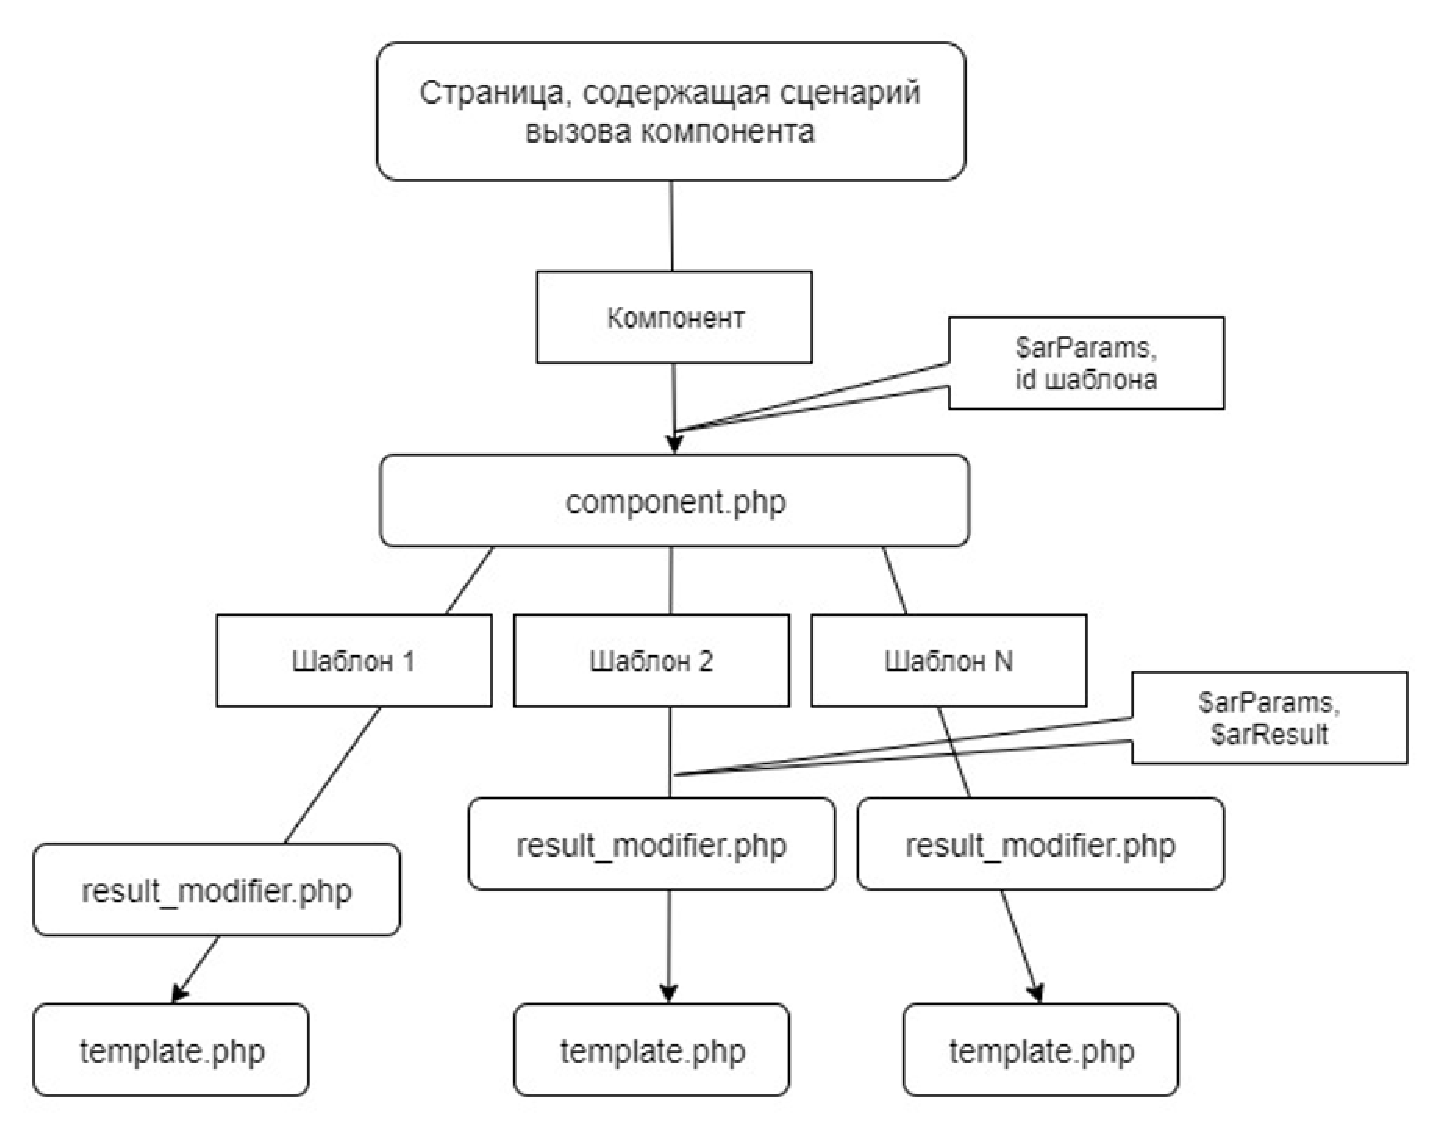
\includegraphics[width=1\linewidth]{data}}
\caption{Диаграмма компонентов}
\label{data:image}
\end{figure}

При вызове компонента в сценарии системы тестирования указывается значения имя пользователя и набор вопросов соответствующий выбранному тесту, которые далее посредством ссылок на объекты классов, описывающих данную информацию \$arParams передаются в следующее окно.

В зависимости от типа вопроса инициализируется соответствующее отображение с вариантами ответа.

Работа компонента заканчивается в момент закрытия главного окна.

\subsection{Диаграмма размещения}

Диаграмма размещения (рис.~\ref{place:image}) отражает физические взаимосвязи между программными и аппаратными компонентами системы.

\vspace{-8mm} % чтобы убрать пустую строку, которая осталась после переноса рисунка на следующую страницу
\begin{figure}[ht]
\center{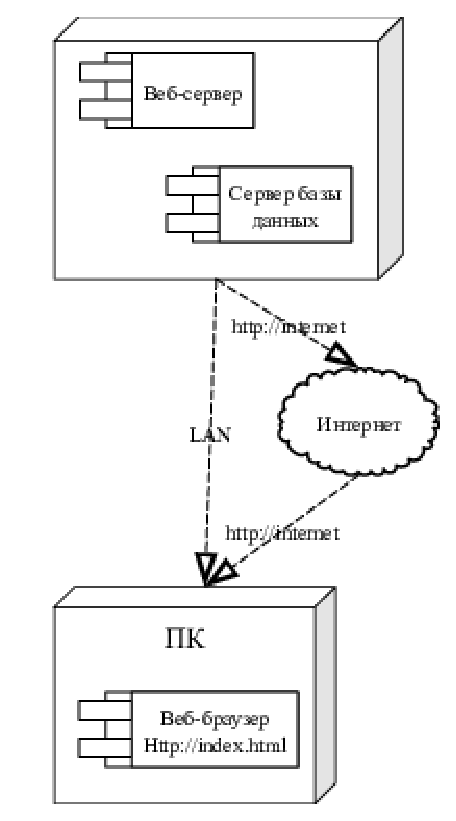
\includegraphics[width=0.57\linewidth]{place}}
\caption{Диаграмма размещения. Не помещается на страницу. Очень длинный заголовок}
\label{place:image}
\end{figure}

Она является хорошим средством для показа маршрутов перемещения объектов и компонентов в распределенной системе.

В таблице \ref{ssevsws:table} приведен пример использования пакета xltabular с автоматическим расчетом ширины столбца.

\begin{xltabular}{\textwidth}{|c|X|X|}
	\caption{Сравнение протоколов SSE и WebSocket\label{ssevsws:table}}\\ \hline
	~  & \centrow  SSE & \centrow WebSocket \\ \hline
	\endfirsthead
	\continuecaption{Продолжение таблицы \ref{ssevsws:table}}
	~ & \centrow SSE & \centrow WebSocket \\ \hline 
	\finishhead
	Направленность & 
	Однонаправленный, полудуплексный: данные посылает только сервер & 
	Двунаправленный, полнодуплексный: и сервер, и клиент могут обмениваться сообщениями \\ \hline 
	Соединение  & HTTP & WS \\ \hline 
	Тип данных & Только текст & Бинарные и текстовые данные \\ \hline 
	Доп. возможности & Встроенный механизм идентификаторов событий и переподключения & Переподключение и идентификация события реализуются на стороне приложения
\end{xltabular}

\subsection{Содержание информационных блоков. Основные сущности}

Проанализировав требования, можно выделить шесть основных сущностей:
\begin{itemize}
\item "<Пользователь">;
\item "<Вопрос">;
\item "<Ответ">;
\item "<Тест">;
\item "<Результат">;
\item "<Диагноз">;
\end{itemize}

В состав сущности "<Пользователь"> можно включить атрибуты, представленные в таблице \ref{news:table}.

\begin{xltabular}{\textwidth}{|l|l|p{1.7cm}|X|}
	\caption{Атрибуты сущности "<Новости">\label{news:table}}\\ \hline
	\centrow Поле & \centrow Тип & \centrow Обяза\-тельное & \centrow Описание \\ \hline
	\thead{1} & \thead{2} & \centrow 3 & \centrow 4 \\ \hline
	\endfirsthead
	\continuecaption{Продолжение таблицы \ref{news:table}}
	\thead{1} & \thead{2} & \centrow 3 & \centrow 4 \\ \hline
	\finishhead
	\_id & ObjectId & true & Уникальный идентификатор \\ \hline 
	head & String & true & Заголовок новости \\ \hline 
	short & String & false & Аннотация к новости \\ \hline 
	createdAt & Date & true & Время создания новости \\ \hline 
	author & String & false & Автор новости \\ \hline 
	content & String & true & Текст новости \\ \hline 
	views & Integer & true & Количество просмотров новости зарегистрированными пользователями
\end{xltabular}

Пример использования различных типов столбцов представлен в таблице \ref{prod:table}. Рекомендуется использовать пакет xltabular для создания таблиц.

\begin{xltabular}{\textwidth}{|R|C{2.5cm}|l|T|}
	\caption{Атрибуты  сущности "<Новости разметки в LaTeX"> с использованием различных типов столбцов и многострочным заголовком\label{prod:table}}\\ \hline
	\centrow Поле & \centrow Тип & \centrow Обязательное & \centrow Описание \\ \hline
	\centrow 1 & \centrow 2 & \thead{3} & \centrow 4 \\ \hline
	\endfirsthead
	\continuecaption{Продолжение таблицы \ref{prod:table}}
	\centrow 1 & \centrow 2 & \thead{3} & \centrow 4 \\ \hline
	\finishhead
	\_id & ObjectId & true & Уникальный идентификатор \\ \hline 
	head & String & true & Заголовок новости \\ \hline 
	short & String & false & Аннотация к новости \\ \hline 
	createdAt & Date & true & Время создания новости \\ \hline 
	author & String & false & Автор новости \\ \hline 
	content & String & true & Текст новости \\ \hline 
	views & Integer & true & Количество просмотров новости зарегистрированными пользователями
\end{xltabular}

В системе предусмотрен внутренний механизм связи между разделами и элементами информационных блоков, поэтому введения дополнительных идентификаторов при реализации связей между сущностями не предполагается.

Экземпляры сущностей реализуются в информационных блоках посредством элементов, атрибуты сущности – посредством полей и свойств элемента. 
